\documentclass[a4paper,10pt]{article}

\usepackage[T1]{fontenc}
\usepackage[utf8]{inputenc}
\usepackage{mathtools}
\usepackage{graphicx}
\usepackage[margin=1in]{geometry}
\usepackage[spanish,activeacute]{babel}
\usepackage{hyperref}
\usepackage{fancyhdr}
\usepackage{incgraph,tikz}
\pagestyle{fancy}

\usepackage{color}
\usepackage{listings}
\lstset{ %
basicstyle=\footnotesize,       % the size of the fonts that are used for the code
numbers=left,                   % where to put the line-numbers
numberstyle=\footnotesize,      % the size of the fonts that are used for the line-numbers
stepnumber=1,                   % the step between two line-numbers. If it is 1 each line will be numbered
numbersep=10pt,                  % how far the line-numbers are from the code
backgroundcolor=\color{white},  % choose the background color. You must add \usepackage{color}
showspaces=false,               % show spaces adding particular underscores
showstringspaces=false,         % underline spaces within strings
showtabs=false,                 % show tabs within strings adding particular underscores
frame=single,           % adds a frame around the code
tabsize=4,          % sets default tabsize to 2 spaces
captionpos=b,           % sets the caption-position to bottom
breaklines=true,        % sets automatic line breaking
breakatwhitespace=false,    % sets if automatic breaks should only happen at whitespace
escapeinside={\%*}{*)}          % if you want to add a comment within your code
}
\renewcommand{\lstlistingname}{Código}
\usepackage{float}
\restylefloat{table}
\makeatletter
\def\verbatim{\small\@verbatim \frenchspacing\@vobeyspaces \@xverbatim}
\makeatother

\title{Speaker Recognition}

\lhead{Métodos Numéricos Avanzados}
\rhead{Análisis Armónico: Speaker Recognition}

\begin{document}

\begin{center}
\textbf{\Huge{Speaker Recognition}}
\end{center}

\begin{center}
\textbf{INTEGRANTES: Meola Franco Román, Puente Julieta, Strubolini Diego Martín}

\textbf{ITBA Segundo Cuatrimestre 2014}
\end{center}

\begin{center}
\text{PALABRAS CLAVE: análisis armónico, speaker recognition, mfcc, transformada de fourier, mel-cepstral }
\end{center}

\begin{center}
\begin{large}
Resumen
\end{large}
\end{center}

Este Trabajo Práctico Especial muestra una posible implementación de un reconocedor de habla en Octave basándonos en la transformada de Fourier para el cálculo de los coeficientes mel-cepstrales de distintas muestras de voz.


\section{Introducción}
El reconocimiento de habla automatizado por una máquina ha sido estudiado por décadas. Hay distintas formas de representaciones paramétricas para señales de acústica. Uno de los más usados es el MFCC o Mel-Frecuency Ceptrum. En el siguiente informe nos basaremos en el paper \textit{An efficient mfcc extraction method in speech recognition} de Wei Han, Cheong-Fat Chan, Chiu-Sing Choy, y Kong-Pang Pun (Ver [1]) y detallaremos una implementación propia en el lenguaje matemático Octave.

\section{Implementación}
Siguiendo los pasos de [1], detallaremos a continuación las principales funciones implementadas para obtener los coeficientes mel-cepstrales.
\newline

\begin{figure}[h]
\centering
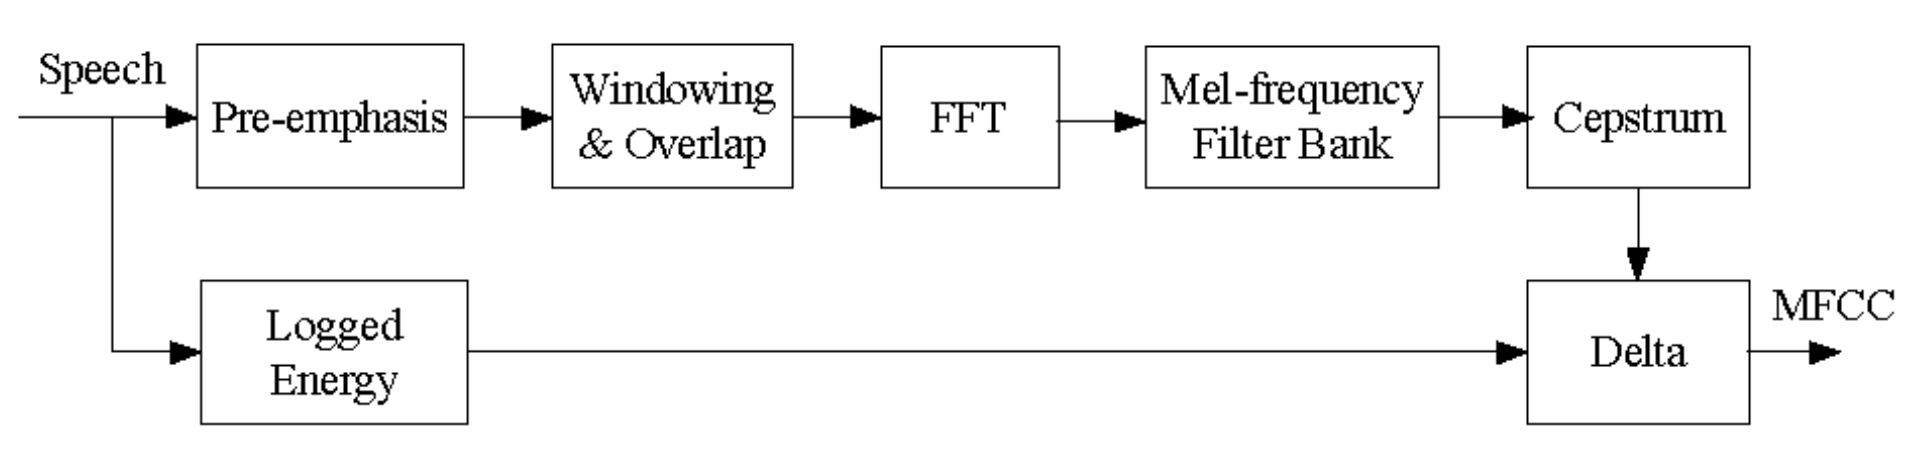
\includegraphics[width=\textwidth]{diagram}
\caption{Diagrama de Trabajo}
\end{figure}

\subsection{Pre-emphasis}

En esta primera función obtendremos un aplanamiento de la señal. Tanto la constante \texttt{a} elegida para este procedimiento (Ver línea 3), como su implementación es similar a la enunciada en la fórmula (1) de [1].
%\cite{han}
\newline
\begin{lstlisting}[language=Octave, caption = Pre-emphasis]
function yp = preemphasis(y, rows)

a = 0.97;
yp(1) = y(1);

for n = 2:rows
	yp(n) = y(n) - a * y(n-1);
end

yp;
\end{lstlisting}

\subsection{Windowing and Overlap}
Esta etapa nos ayuda a reducir los cambios bruscos del principio y fin de la trama en donde va de cero a la señal y de la señal a cero respectivamente.
Para esta función también utilizamos los mismos valores que en [1]. En la misma recibimos el vector de Hamming para ahorrarnos el cálculo del mismo en cada iteración. En la línea 5 utilizamos el vector de Hamming generado por el método \texttt{hamming} de Octave.
\newline
\begin{lstlisting}[language=Octave, caption = Windowing]
function yw = windowing(y,frameSize,frameNmb,overlap,hamming)

i=1;
for k=1 + overlap*(frameNmb -1) : frameSize + overlap*(frameNmb-1)
	yw(i)=y(k)*hamming(i);
	i=i+1;
end

yw;
\end{lstlisting}

\subsection{FFT}

Para el cálculo de la transformada de Fourier utilizamos el método \texttt{fft} provisto por Octave. Éste método utiliza la Transformada Rápida de Fourier vista en clase.

\subsection{Mel-frequency Filter Bank}

En esta etapa tomamos como referencia el tutorial sugerido por la cátedra [4]. En la función \texttt{filterbanks} de [4] se obtienen 26 filtros, pero en nuestro caso elegimos utilizar 33 filtros como en la descripción de [1]. Por el mismo motivo utilizamos 256 puntos de la transformada de Fourier obtenida en la etapa anterior. 
Luego de revisar los detalles de [4] decidimos utilizar 300 como el valor del parámetro \texttt{min}, ya que usando 0 (como sugiere [1]) no obtuvimos los resultados esperados.
\newline
\begin{lstlisting}[language=Octave, caption = filterbanks]
function fb = filterbanks(min,max,amount,fftsize)

mmax = mel(max);
mmin = mel(min);
step = (mmax-mmin)/(amount+1);

for k=1:amount+2
	num = (k-1)*step + mmin;
	f(k) = num;
	fm(k) = melinv(num);
	fb(k) = floor((fftsize+1)*fm(k)/(max*2));
end

fbank = zeros(amount,fftsize/2+1);

for j=1:amount
	for i=fb(j):fb(j+1)
		fbank(j,i) = (i - fb(j))/(fb(j+1)-fb(j));
	end
	for i=fb(j+1):fb(j+2)
		fbank(j,i) = (fb(j+2)-i)/(fb(j+2)-fb(j+1));
	end
end

fb = fbank;
fb;
\end{lstlisting}
El ciclo \texttt{for} de la línea 16 fue extraído de la implementación en Python de [4].

\subsection{Cepstrum}

En el siguiente ciclo calculamos los primeros 12 coeficientes mel-cepstrales. En el mismo utilizamos la ecuación (4) de [1].
\newline
\begin{lstlisting}[language=Octave, caption = Extracto de la función mfcc]
for n = 1 : (coef_amount - 1)
	c = 0;
	for k = 1 : filter_amount
		c += log(filterenergies(k))*cos(n*(k-0.5)*pi/filter_amount);
	end
	coef(n) = c;
end
\end{lstlisting}

\subsection{Logged Energy}
Para calcular el décimo-tercer coeficiente mel-cepstral utilizamos la función (5) de [1].
\newline
\begin{lstlisting}[language=Octave, caption = Logged Energy]
function energy = loggedenergy(y,framesize)

energy = 0;
for n = 1 : framesize
	energy += y(n)**2;
end;

energy = log(energy);	
energy;
\end{lstlisting}

\subsection{Deltas}
En esta etapa obtuvimos los otros trece coeficientes (coeficientes deltas) para lograr el total de veintiséis coeficientes \texttt{mfcc} necesarios utilizando la función (6) de [1].
Luego de solicitar asistencia a la cátedra, en los casos extremos donde el índice se va de rango se utilizó el vector nulo.
\newline

\begin{lstlisting}[language=Octave, caption = Extracto de la función mfcc]
delta(1,:) = (2*(mfcc(:,3)) + (mfcc(:,2)))/10;
delta(2,:) = (2*(mfcc(:,4)) + (mfcc(:,3) - mfcc(:,1)))/10;
for f = 3 : (total_frames-2)
	delta(f,:) = (2*(mfcc(:,f+2) - mfcc(:,f-2)) + (mfcc(:,f+1) - mfcc(:,f-1)))/10;
end
delta(total_frames-1,:) = (2*(-1*mfcc(:,total_frames-3)) + (mfcc(:,total_frames) - mfcc(:,total_frames-2)))/10;
delta(total_frames,:) = (2*(-1*mfcc(:,total_frames-2)) + (-1*mfcc(:,total_frames-1)))/10;
\end{lstlisting}

\subsection{MeanDist y VQ}
Luego de obtener los coeficientes \texttt{mfcc} de cada trama se extrajeron 16 vectores representativos a partir de la función \texttt{vq}.  
Estos vetores se compararon con los \texttt{mfcc} de los audios de entrenamiento, utilizando la función \texttt{meandist} provista por la cátedra.

\section{Resultados}
Luego de probar todos los audios de prueba y comparándolos con los audios de prueba obtuvimos los siguientes resultados. En las tablas detallamos:
\begin{itemize}
\item Persona: el nombre de la persona que grabó el audio de prueba.
\item Coincidencia: Si el programa identificó correctamente el audio de entrenamiento.
\item Falsa Coincidencia: En caso de no haber coincidencia se indica el nombre de la persona que el programa asumió.
\end{itemize}
Se muestran los resultados para las frases de prueba "$Susana"$ y "$Juan"$.
\begin{center}
\begin{table}[h]
\centering
\begin{tabular}{ccc}
\hline
\textbf{Persona} & \textbf{Coincidencia} & \textbf{Falsa Concidencia} \\ \hline
Franco&No&Enzo\\
Sandra&Si&-\\
Enzo&Si&-\\     
Paula&Si&-\\     
Diego&Si&-\\ 
Monica&No&Julieta\\
Julieta&No&Sandra\\
Daniela&No&Juli\\
Agostina&No&Sandra\\
Sebastián&Si&-\\
\end{tabular}
\caption[Texto del índice (opcional)]{Susana: 50\% de efectividad}
\end{table}
\end{center}

\begin{center}
\begin{table}[h]
\centering
\begin{tabular}{ccc}
\hline
\textbf{Persona} & \textbf{Coincidencia} & \textbf{Falsa Concidencia} \\ \hline
Franco&No&Sandra\\
Sandra&No&Enzo\\
Enzo&Si&-\\     
Paula&Si&-\\     
Diego&Si&-\\ 
Monica&No&Julieta\\
Julieta&Si&-\\
Daniela&Si&-\\
Agostina&No&Julieta\\
Sebastián&Si&-\\
\end{tabular}
\caption[Texto del índice (opcional)]{Juan: 60\% de efectividad}
\end{table}
\end{center}

Como se puede ver la efectividad es mayor al 50\%, lo que consideramos un resultando decente pero no ideal. Hay que tener en cuenta que si tomamos como acertada la elección de cualquier miembro de la familia y del mismo sexo para un sujeto de prueba, la tasa de efectividad aumenta a un 80\%. Esto se ve reflejado en las pruebas de Enzo con Franco (Padre e Hijo), Mónica y Julieta (Madre e Hija) y Agostina con Julieta (Hermanas). Asumimos que la frecuencia entre voces de una misma familia, siendo las mismas de mismo sexo, son similares.

\section{Problemas Encontrados}
Uno de los principales problemas encontrados fue que con ciertos archivos de audio los vectores generados por nuestra implementación variaban considerablemente en dimensión, lo que generaba problemas de rangos inválidos. Una de las características que encontramos en común entre estos archivos eran que contenían silencios absolutos en el medio, lo que suponemos fue la causa de estos problemas.

\section{Conclusiones}
Como conclusión y para terminar, creemos que deberíamos haber elegido frases de prueba de mayor longitud (no de una sola palabra). Decidimos trabajar con frases cortas para reducir el tiempo de procesamiento de la función, que luego nos dimos cuenta que sacrificó efectividad. Si bien, en un principio esperábamos tasas de efectividad más altas a las conseguidas, los resultados conseguidos siguen siendo mejores a una simple elección aleatoria.

\begin{thebibliography}{9}
\bibitem{han} Wei Han, Cheong-Fat Chan, Chiu-Sing Choy, and Kong-Pang Pun. An efficient mfcc extraction method in speech recognition. In Proceedings IEEE International Symposium on Circuits and Systems, 2006. ISCAS 2006., pa- ges 4 pp.–, May 2006.
\bibitem{hasan} Md Rashidul Hasan, Mustafa Jamil, Md Golam Rabbani, and Md Saifur Rahman. Speaker identification using mel frequency cepstral coefficients. In 3rd International Conference on Electrical \& Computer Engineering ICECE, volume 2004, 2004.
\bibitem{linde} Y. Linde, A Buzo, and R.M. Gray. An algorithm for vector quantizer design. IEEE Transactions on Communications, 28(1):84–95, Jan 1980.
\bibitem{} James Lyons. Mel frequency cepstral coefficient (mfcc) tutorial. 
\url{http://practicalcryptography.com/miscellaneous/machine-learning/guide-mel-frequency-cepstral-coefficients-mfccs/}
\bibitem{} Manual de Funciones de Octave \url{https://www.gnu.org/software/octave/doc/interpreter/}
\end{thebibliography}

\section{Funciones Auxiliares}

\begin{lstlisting}[language=Octave, caption = Mel]
function m = mel(f)

m = 1125*log(1+f/700);

m;
\end{lstlisting}

\begin{lstlisting}[language=Octave, caption = Mel Inversa]
function m = melinv(f)

m = 700*(exp(f/1125)-1);

m;
\end{lstlisting}

\begin{lstlisting}[language=Octave, caption = Periodogram]
function yp = periodogram(y,frameSize)

for k=1 : frameSize
  yp(k)= (abs(y(k))**2)/frameSize;
end

yp;
\end{lstlisting}

\pagebreak

\tableofcontents

\end{document}